\chapter{Experiments and results}\label{result}
In this chapter, the evaluation criteria are presented first. 
Then, the experiments regarding I2I translation are depicted.
Subsequently, two experiments are conducted to explore the use of I2I techniques for improving segmentation.
\section{Evaluation Criteria}
In order to select which images are used for training the segmentation network, metrics should be used in addition to qualitative human evaluation.
Traditional evaluation metrics such as the accuracy and precision of the models are not fitting for evaluating GANs, as there is no ground truth to compare the generated data to.
Researchers have developed different approaches to overcome this challenge.
One of the most popular GAN evaluation metrics to evaluate the generated images is the Frechet Inception Distance (FID) \cite{alqahtani2019analysis}.
A different approach would be the Structural Similarity Index Measure (SSIM), which measures the image quality by comparing an original and a generated image. 
It was introduced by Wang et al. \cite{wang2004image}.
\paragraph{Fréchet inception distance}
The FID was introduced by Heusel et al. \cite{heusel2017gans} as a performance measure for GANs, which measures the similarity between two sets of images, in this case, the generated and the original images.
It is based on extracting high-level information from a generated and an original image by passing it through an Inception model.
The output features are then compared by the Fréchet distance.\\
The Inception model as proposed in \cite{szegedy2015going} is a deep CNN, which introduces inception modules.
These inception modules feature parallel convolution operations with different filter sizes to capture features at different scales, of which the results are concatenated and used as input for the next layer.
The inception blocks are then repeated to capture increasingly complex and abstract features.\\
To make the resulting vision-relevant features comparable, the mean and covariance over the set of the feature vectors of each image are calculated respectively.
It is assumed that the features follow a multidimensional Gaussian distribution with mean and covariance of the features \cite{heusel2017gans}.
The resulting distributions $F$ of an original and $G$ for a generated image are then compared using the Fréchet inception distance $d^2$ as defined in equation \ref{fid}, according to \cite{dowson1982frechet}:
\begin{equation}
    d^2(F,G) = |\mu_F - \mu_G|^2 + \text{Tr}(\Sigma_F + \Sigma_G - 2\sqrt{\Sigma_F \Sigma_G}),
    \label{fid}
\end{equation}
where $\text{Tr}$ denotes the trace operator, $\mu$ the mean, and $\Sigma$ the covariance matrix of the respective distribution.
The FID is typically calculated by computing the mean and covariance over a set of generated images and a set of original images separately and then using these values to measure the distance between the distributions using the Fréchet distance.
A lower FID score indicates that the two sets of images are more similar.

\paragraph*{SSIM}
The SSIM measure is based on the measurement of structural content $s$, luminance $l$, and contrast $c$. 
These values for an original image $x$ and a generated image $y$ can be compared as defined in equation \ref{ssim_l}, \ref{ssim_s}, and \ref{ssim_c}, according to~\cite{wang2004image}.
\begin{equation}
    l(x, y) =  \frac{2\mu_x\mu_y + C_1}{\mu^2_x + \mu^2_y + C_1}
    \label{ssim_l}
\end{equation}
\begin{equation}
    c(x, y) =  \frac{2\sigma_x\sigma_y + C_2}{\sigma^2_x + \sigma^2_y + C_2}
    \label{ssim_s}
\end{equation}
\begin{equation}
    s(x, y) =  \frac{2\sigma_{xy} + C_3}{\sigma_x\sigma_y + C_3}
    \label{ssim_c}
\end{equation}
Hereby, $\sigma$ denotes the standard deviation, $\mu$ the mean of the corresponding image, and the $C$ values a constant to improve numerical stability. 
The three measures are combined to the SSIM as defined in equation \ref{ssim_eq}, according to~\cite{wang2004image}.
\begin{equation}
    \text{SSIM}(x, y) = [l(x,y)]^\alpha \cdot [c(x,y)]^\beta \cdot [s(x,y)]^\gamma
    \label{ssim_eq}
\end{equation}
The parameters $\alpha$, $\beta$, and $\gamma$ regulate the influence of the individual measures. 
Hereby, a SSIM score of 1 means that the two images are identical regarding their structural information, while a score of 0 indicates no structural similarity at all.

\paragraph{Intersection Over Union and Dice Similarity Coefficient}
Two metrics that have proven to be effective for the segmentation of surgical tools are the Dice Similarity Coefficient and the Jaccard index \cite{leifman2022pixel}.
The Jaccard index as described in equation \ref{jaccard_index} is also known as the Intersection Over Union (IoU).
As a popular metric, it is used to evaluate the segmentation results.
For a pixel-wise prediction of the classes in an image, it can be implemented as adapted from \cite{leifman2022pixel}:
\begin{equation}
    \text{IoU}(A,B) = \frac{\sum_{i=1}^{|A|} a_i b_i}{\sum_{i=1}^{|A|} (a_i + b_i - a_i b_i)}
\end{equation}
for two binary segmentation masks $A$ and $B$ of the same size with the respective values $a$ and $b$ for each pixel position $i$.
Thereby, $a$ and $b$ have a value of 0 for background and 1 if the class for which the metric is calculated occurs there.
Another way of calculating this metric is with a confusion matrix, where all true positives (TP), false positives (FP), true negatives (TN), and false negatives (FN) are calculated for each prediction and ground truth of the segmentation masks.
The IoU for a class $c$ can be calculated as described in \cite{sulistiyo2018attribute}:
\begin{equation}
     \text{IoU}_c = \frac{\text{TP}_c}{\text{TP}_c + \text{FP}_c + \text{FN}_c}
\end{equation}
This is calculated for each class of surgical instruments that occur in the data of the current task.
To get the mean IoU (mIoU) for the whole data, the IoU values for each class are summed and then divided by the number of classes $C$:
\begin{equation}
    \text{mIoU} = \frac{1}{C}\sum_{i=1}^{C} \frac{\text{TP}_c}{\text{TP}_c + \text{FP}_c + \text{FN}_c}
\end{equation}
The IoU for the background is not included, because it is considered not a relevant class.\\
The Dice Similarity Coefficient also measures the overlap between the predicted segmentation mask and the ground truth mask.
It is calculated as twice the intersection of the predicted and ground truth masks divided by the sum of their areas.
The Dice Similarity Coefficient is defined as in \cite{leifman2022pixel}:
\begin{equation}
    D(A,B) = \frac{2|A \cap B|}{|A| + |B|}
\end{equation}
Thus, using true positives and false negatives, the Dice coefficient can be defined as follows:
\begin{equation}
    \text{Dice} = \frac{2\text{TP}}{2\text{TP} + \text{FP} + \text{FN}}
\end{equation}
Therefore, the mean Dice (mDice) can be calculated as:
\begin{equation}
    \text{mDice} = \frac{1}{C}\sum_{i=1}^{C} \frac{2\text{TP}_c}{2\text{TP}_c + \text{FP}_c + \text{FN}_c}
\end{equation}
Both, IoU and Dice range from zero to one with zero indicating no overlap between the predicted and ground truth masks, while a value of one represents complete overlap between the two masks.
% was sind gute scores für miou
% was sind gute scores für dice

\section{Image to image translation}\label{i2i_trans}
In this section the CycleGAN and StarGAN architecture are used to translate images into images with artificial smoke.
\subsection{CycleGAN}\label{cyclegan_experiment}
A CycleGAN with an architecture as described in section \ref{cyclegan} is used to translate images from the no-smoke domain to the heavy-smoke domain.
Also, the identity loss was used for training the CycleGAN, because it seems to help preserve the overall structure of the image. 
Adam is used to optimize the generators and discriminators to speed up the convergence of both networks and improves the overall performance of the CycleGAN.
Hereby the beta values are set to 0.5 for $\beta_1$ and 0.999 for $\beta_2$.\\
An image buffer, which holds up to 20 images is implemented to reduce the oscillation in the training process.
A one-cycle scheduler as proposed in \cite{smith2018disciplined} is used for adjusting the learning rate during training for faster convergence of the network.
The learning rate starts hereby at a lower value, increases to the maximum set value in the middle of the training process, and then decreases again towards the end of the training, shown exemplarily in Figure \ref{one_cycle}.
For implementation, the Pytorch OneCycleLR is used with a percentage start (pct) of 0.05 meaning the learning rate will increase for the first five percent of the total amount of steps and afterward starts decreasing.
An example of the adjustment of the learning rate is given in Figure \ref{one_cycle}.
\begin{figure}[tb]
    \begin{center}
     \includegraphics[width=8cm]{./images/once_cycle.pdf}
    \caption[One-cycle scheduler]{{Exemplary learning rate adjustment with one-cycle scheduler for 86,190 steps and pct start of 0.05.
    }\label{one_cycle}}
    \end{center}
\end{figure}
\paragraph*{Data} 
The generated images should be in the heavy-smoke domain because it is assumed that this will have the greatest benefit in training the segmentation.
The images which are translated are from the no-smoke domain as these are the most present.
Therefore the training data consists of images from the no- and heavy-smoke domains.
The dataset for training returns a batch of random pairs of these domains.
Because of the tanh activation function used in this model, the image values have to be in the same range of [-1,1] as tanh.
This is done by dividing the pixel values by the maximal pixel value of 255.
Then they are normalized with a mean and standard deviation of 0.5.
Therefore the generated images are in the same value range as the original ones.
Otherwise, the discriminator could detect the original images based on value outliers.\\
Due to computational limitations, the images are downsized by a factor of two.
The original images are in a resolution of $1920\times1080$ pixels, so they are downsized to $960\times540$.
Because for the validation of the segmentation network a six-fold cross-validation is used, the same folds should be used for training the CycleGAN to not introduce information about the validation data.
The training data for each fold contains the images of five out of the six videos.
In the following, training fold one means omitting video one, and therefore videos two to six are used for training. 
\paragraph{Hyperparameters} The hyperparameters for the model are chosen as follows.
A batch size of two is used due to memory limitations.
To initialize the model, all of the weights were set to values from a Gaussian distribution $N(0, 0.02)$, which has been found to be a suitable starting point for this particular architecture \cite{Zhu2017}.
The learning rate of the generator and discriminator is set to $10^{-4}$, which is the highest learning rate, where the networks converge to a stable equilibrium. 
Adopted from the original CycleGAN the lambda values for the cycle-consistency loss are set to ten and the lambda for the identity loss to five.\\
\paragraph*{Training}
\begin{figure}[bt]
    \centering
    \subfloat[Loss of discriminator for no-smoke images.]{\includegraphics[width=0.49\textwidth]{./images/plots_cyclegan/disc_ns_loss.pdf}\label{fig:disc_ns_loss}}
    \hfill
    \subfloat[Loss of discriminator for heavy-smoke images.]{\includegraphics[width=0.49\textwidth]{./images/plots_cyclegan/disc_hs_loss.pdf}\label{fig:disc_hs_loss}}
    
    \vspace{0.5cm}
    
    \subfloat[Loss of generator for no-smoke images.]{\includegraphics[width=0.49\textwidth]{./images/plots_cyclegan/gen_ns_loss.pdf}\label{fig:gen_ns_loss}}
    \hfill
    \subfloat[Loss of generator for heavy-smoke images.]{\includegraphics[width=0.49\textwidth]{./images/plots_cyclegan/gen_hs_loss.pdf}\label{fig:gen_hs_loss}}
    
    \caption[CycleGAN loss curves]{Display of the loss values for the domain-specific generator and discriminator during training.}\label{fig:cycle_disc_gen_loss}
\end{figure}
The model was trained for 30 epochs, as no further improvement of the generated data was observed afterward.
Figure \ref{fig:cycle_disc_gen_loss} displays the change in the discriminator and generator loss during training, with values averaged over one epoch, whereby in the individual steps, the oscillation is much higher.
The generators and discriminators converge around epoch seven.
The loss value for the discriminator saturates at around 0.4, which is a value that provides enough information for the generator to learn how to fool the discriminator, while still penalizing images that are too far from the original image distribution.\\
Due to its architecture, the CycleGAN produces artificial images of both domains, heavy-smoke and no-smoke.
The evaluation of these is focused on the heavy-smoke images only, because they are the only ones used to enhance the segmentation training.
To evaluate the generated images the FID is computed by comparing the Gaussian distributions of the generated heavy-smoke images with the distribution of original heavy-smoke images because the similarity of the images should be tested not only regarding the general structure but also regarding the occurrence of smoke.
Therefore, the mean and standard deviation of both the generated and original images are updated on a per-image basis, with an equal number of updates applied to each.
After updating the means and standard deviations of the generated and original images for one epoch, the FID between the resulting distributions is calculated.
The SSIM is calculated with one generated and one original heavy-smoke image at once, to set the focus of this metric more on the smoke generation like in the FID.
The resulting values are averaged over one epoch.
The progress of both metrics during training is shown in Figure \ref{fig:cycle_metrics}.
\begin{figure}[tb]
    \centering
    \subfloat[SSIM in CycleGAN training.]{\includegraphics[width=0.49\textwidth]{./images/plots_cyclegan/ssim_cycle.pdf}\label{fig:ssim_cycle}}
    \hfill
    \subfloat[FID in CycleGAN training.]{\includegraphics[width=0.49\textwidth]{./images/plots_cyclegan/fid_cycle.pdf}\label{fig:fid_cycle}}
    \caption[FID and SSIM of CycleGAN]{Display of the FID and SSIM values evaluated every 5 epochs.}\label{fig:cycle_metrics}
\end{figure}
The FID is decreasing for all folds until epoch 20, where it reaches its minimum. 
After that, a slight increase can be seen.
The SSIM grows for fold 5 until epoch 30, fold one and two saturate after epoch 25, and a slight decrease occurs after epoch 20 for fold 3, 4, and 6.
This indicates that the optimum is around epoch 20.
Human evaluation comes to a correlating result, by comparing random generated images in the different epochs as shown in Figure \ref{fig:cycle_img_train}.
\begin{figure}[tb]
    \centering
    \subfloat[Original image.]{\includegraphics[width=0.49\textwidth]{./images/CycleGAN_imgs/f_8550_artifact_org.png}\label{fig:art_o}}
    \hfill
    \subfloat[Generated image after 5 epochs.]{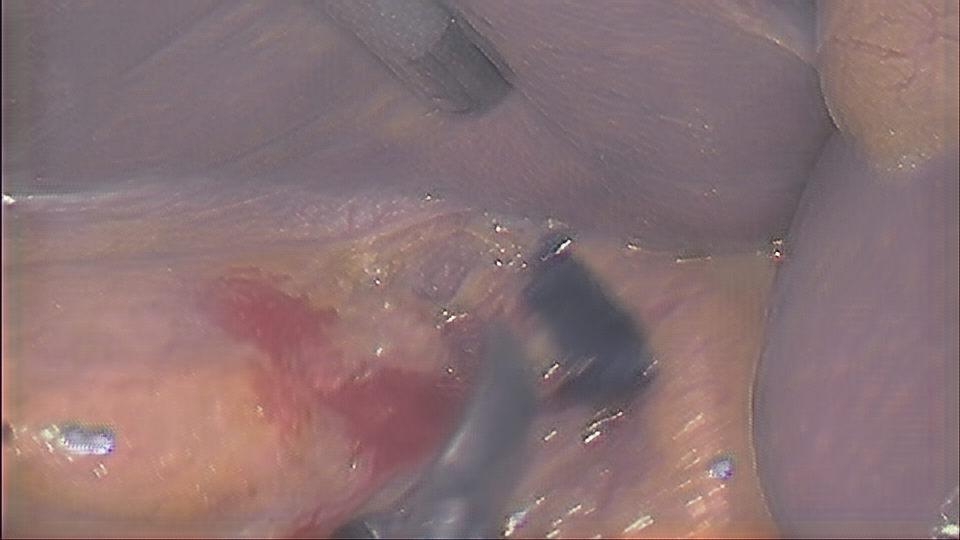
\includegraphics[width=0.49\textwidth]{./images/CycleGAN_imgs/f_8550_artifact_5.png}\label{fig:art_5}}
    
    \vspace{0.5cm}
    
    \subfloat[Generated image after 20 epochs.]{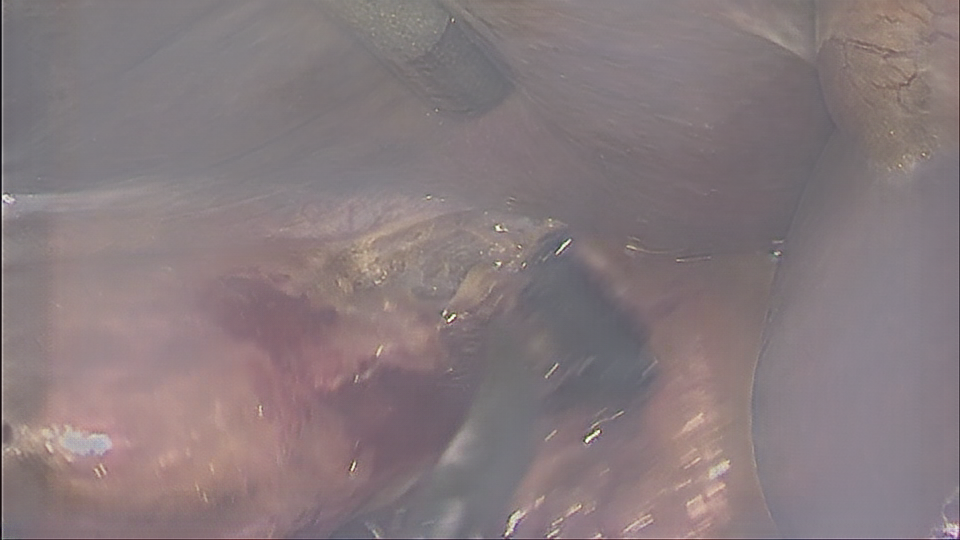
\includegraphics[width=0.49\textwidth]{./images/CycleGAN_imgs/f_8550_artifact_20.png}\label{fig:art_20}}
    \hfill
    \subfloat[Generated image after 30 epochs.]{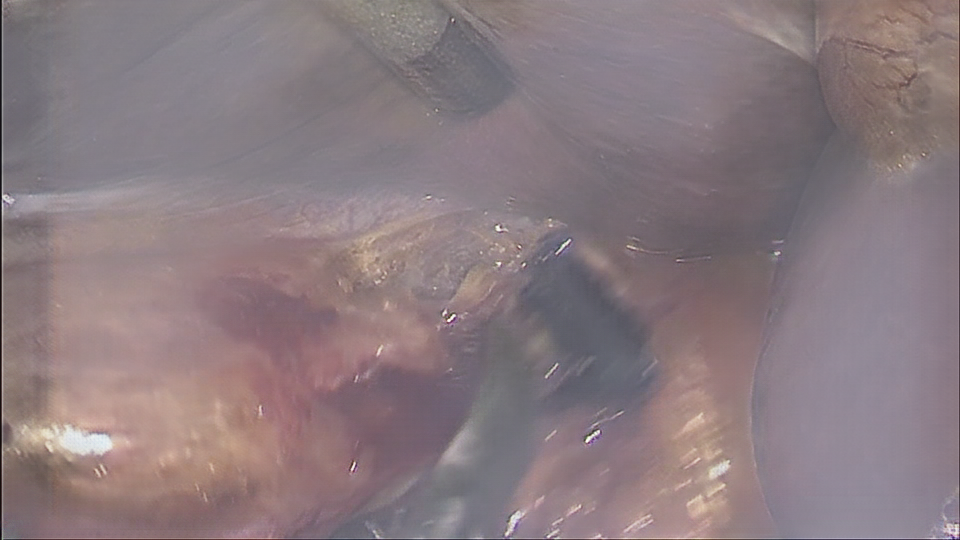
\includegraphics[width=0.49\textwidth]{./images/CycleGAN_imgs/f_8550_artifact_30.png}\label{fig:art_30}}
    \caption[Image generation of CycleGAN]{Image generation process at different epochs, taken from video 6 frame 8550 of fold 2.}\label{fig:cycle_img_train}
\end{figure}
In Figure \ref{fig:art_30} it can be seen, that artifacts like the dark bar on the left side of the image are more prominent than in the previous epochs.
On a different note, in epoch 5 of the generation process also a little artifact around the reflection in the left corner can be seen.
The generated image of epoch 20 seems like a good tradeoff. Additionally, the generated smoke seems a bit more dense than in the other steps.\\
Since metrics like SSIM or FID can also find correlations that are not immediately obvious to the human eye, the metrics should also be taken into account.
Therefore, the images, generated in epoch 20, have been selected as the most optimal representations based on the evaluation metrics and subjective human assessment.
Figure \ref{fig:cycle_showcase} presents a comparison of the generated images with their corresponding originals.
Table \ref{fid_ssim_cycle_table} presents the SSIM and FID values that indicate the best results.
\begin{table}[!tb]\vspace{1ex}\centering
    \caption[Metrics CycleGAN]{FID and SSIM values for evaluation at epoch 20.\label{fid_ssim_cycle_table}}
    \begin{tabular*}{8cm}{ll|@{\extracolsep\fill}cccc}
    &&\multicolumn{2}{c}{Metric} \\
    && FID & SSIM  \\\hline
    %\multirow{6}*{\rotatebox{90}{Domain}}
    & Fold 1 &  39.55  & 0.7860 \\%\cline{2-6}
    & Fold 2 & 44.21  &  0.7749 \\%\cline{2-6}
    & Fold 3 & 40.26  &  0.7891\\%\cline{2-6}
    & Fold 4 & 44.55  &  0.7914\\%\cline{2-6}
    & Fold 5 & 41.42  &  0.7818\\%\cline{2-6}
    & Fold 6 & 41.05 &  0.7844\\\hline
    & mean & 41,84 & 0.7846\\
    \end{tabular*}
    \captionsetup{justification=centering}
\vspace{2ex}\end{table}
\begin{figure}[bt]
    \centering
    \subfloat[Original HS.]{\includegraphics[width=0.25\textwidth]{./images/CycleGAN_imgs/showcase/f_17004_original_smoke.png}\label{fig:org_cycle_1}}
    \hfill
    \subfloat[Original HS.]{\includegraphics[width=0.25\textwidth]{./images/CycleGAN_imgs/showcase/f_18003_original_smoke.png}\label{fig:org_cycle_2}}
    \hfill
    \subfloat[Original HS.]{\includegraphics[width=0.25\textwidth]{./images/CycleGAN_imgs/showcase/f_26006_original_smoke.png}\label{fig:org_cycle_3}}
    \hfill
    \subfloat[Original HS.]{\includegraphics[width=0.25\textwidth]{./images/CycleGAN_imgs/showcase/f_28000_original_smoke.png}\label{fig:org_cycle_4}}
    \vspace{0.5cm}
    \subfloat[Original NS.]{\includegraphics[width=0.25\textwidth]{./images/CycleGAN_imgs/showcase/f_6600_org.png}\label{fig:cycle_org1}}
    \hfill
    \subfloat[Generated HS.]{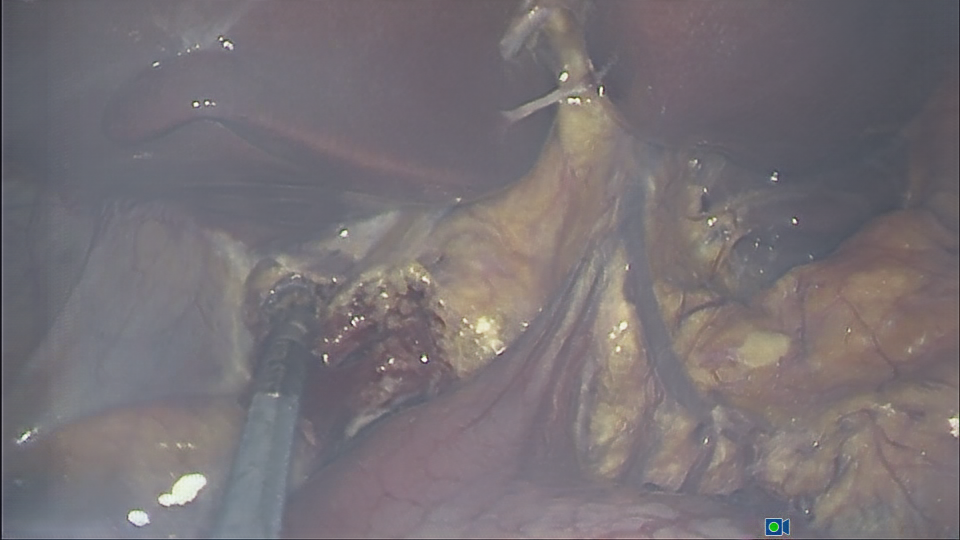
\includegraphics[width=0.25\textwidth]{./images/CycleGAN_imgs/showcase/f_6600.png}\label{fig:cycle_gen1}}
    \hfill
    \subfloat[Original NS.]{\includegraphics[width=0.25\textwidth]{./images/CycleGAN_imgs/showcase/f_7075_org.png}\label{fig:cycle_org2}}
    \hfill
    \subfloat[Generated HS.]{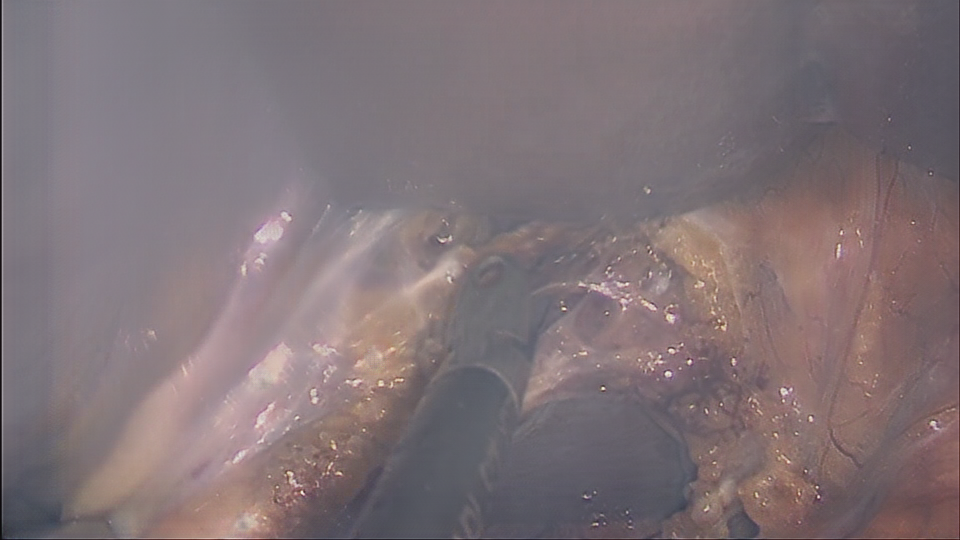
\includegraphics[width=0.25\textwidth]{./images/CycleGAN_imgs/showcase/f_7075.png}\label{fig:cycle_gen2}}
    \vspace{0.5cm}    
    \subfloat[Original NS.]{\includegraphics[width=0.25\textwidth]{./images/CycleGAN_imgs/showcase/f_12150_org.png}\label{fig:cycle_org3}}
    \hfill
    \subfloat[Generated HS.]{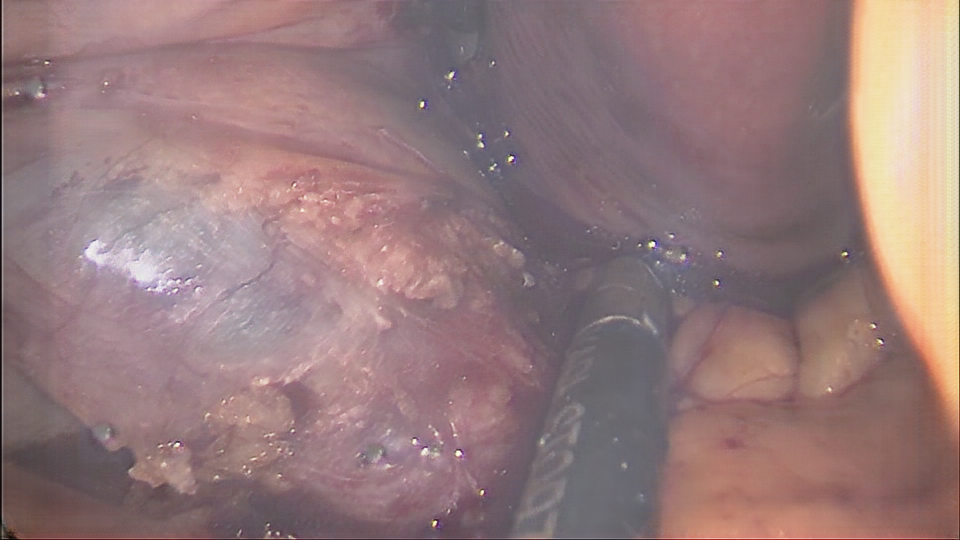
\includegraphics[width=0.25\textwidth]{./images/CycleGAN_imgs/showcase/f_12150.png}\label{fig:cycle_gen3}}
    \hfill
    \subfloat[Original NS.]{\includegraphics[width=0.25\textwidth]{./images/CycleGAN_imgs/showcase/f_12750_org.png}\label{fig:cycle_org4}}
    \hfill
    \subfloat[Generated HS.]{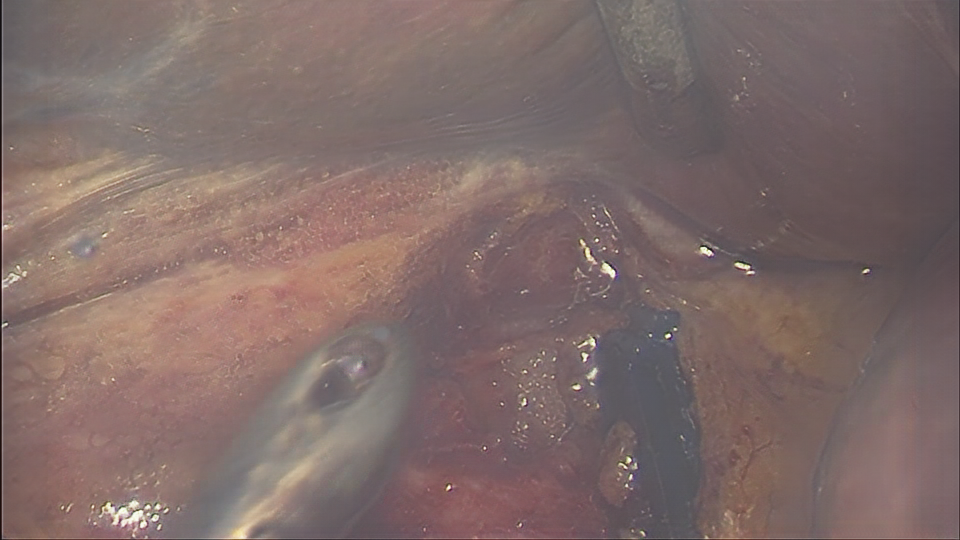
\includegraphics[width=0.25\textwidth]{./images/CycleGAN_imgs/showcase/f_12750.png}\label{fig:cycle_gen4}}
    \vspace{0.5cm}
    \caption[Generated images of CycleGAN.]{(a)-(d) representing original images in the heavy-smoke domain, (e),(g),(i),(k) original images from the no-smoke domain, and (f),(h),(j),(l) generated images from the corresponding original image shown in (e),(g),(i),(k).}\label{fig:cycle_showcase}
\end{figure}
\FloatBarrier
%-> FID und SSIM tabelle?
%-> oszillation nochmal in grafik darstellen
%-> schreiben was ist discriminator loss genau? 
%\clearpage
\subsection{StarGAN}
A StarGAN model is used to generate not only heavy-smoke images but also slight-smoke images due to its ability to translate into multiple domains.
For this, the architecture described in \ref{star_gan} is used.
To preserve the original structure of the image, an identity loss as in the CycleGAN is introduced in addition to the reconstruction loss.
This is done by conditioning the generator to translate an image to its original domain, which should result in the identity of the original image.
This identity is compared to the source image by calculating the mean absolute error and this loss is added to the general objective of the StarGAN.
The use of a one-cycle learning rate scheduler and the Adam optimizer proved to be effective in training the CycleGAN model, which is why they are also used here in the same configuration.\\
Due to its similar generator, the images to be translated are pre-processed in the same way as in the CycleGAN model.
For conditioning, the generator to translate an image to the desired domain, a one-hot encoded vector of length three is defined with position one denoting no smoke, two slight smoke, and three heavy smoke.
This vector is used to compare the results of the discriminators' class prediction to the ground truth and create the input condition matrix, which is concatenated with the input image.
The original images are loaded randomly as no pairing is required due to the conditioning.
\paragraph{Hyperparameters} The hyperparameters for the model are chosen as follows.
Because of its reduced model size a batch size of six is chosen.
The learning rate for the generator and discriminator is set to $2 \cdot 10^{-4}$.
To adjust the influence of the different loss functions, the lambda values used are 10 for the reconstruction loss, 1 for the domain classification loss, 4 for the identity loss, and 10 for the gradient penalty.
The weights of the model are initialized with values from a Gaussian distribution of $N(0, 0.02)$.
\paragraph{Training} The training consisted of optimizing the model parameters for 30 epochs, whereby the images are loaded in random order in a batch.
The target domain of each image is assigned randomly, whereby the source domain of the image won't be chosen.
Figure \ref{fig:star_train} shows the loss of the generator and discriminator.
\begin{figure}[tb]
    \centering
    \subfloat[Generator with reconstruction loss and classification loss]{\includegraphics[width=0.33\textwidth]{./images/plot_stargan/g_loss_star.pdf}\label{fig:g_star}}
    \hfill
    \subfloat[Generator loss only.]{\includegraphics[width=0.33\textwidth]{./images/plot_stargan/g_loss_oscill_star.pdf}\label{fig:g_star_oscil}}
    \hfill
    \subfloat[Generated class loss.]{\includegraphics[width=0.33\textwidth]{./images/plot_stargan/g_loss_class_star.pdf}\label{fig:g_star_class}}
    
    \vspace{0.5cm}
    
    \subfloat[Discriminator loss fake \\ images.]{\includegraphics[width=0.33\textwidth]{./images/plot_stargan/d_loss_fake_star.pdf}\label{fig:d_star_fake}}
    \hfill
    \subfloat[Discriminator loss original images.]{\includegraphics[width=0.33\textwidth]{./images/plot_stargan/d_loss_real_star.pdf}\label{fig:d_star_real}}
    \hfill
    \subfloat[Discriminator class loss.]{\includegraphics[width=0.33\textwidth]{./images/plot_stargan/d_loss_class_star.pdf}\label{fig:d_star_class}}
    \caption{Loss representations during the training of StarGAN.}\label{fig:star_train}
\end{figure}
Hereby the combined generator loss shown in Figure \ref{fig:g_star} includes the identity and reconstruction loss, which, when decreasing as in this case, indicates a working training.
The generator loss in Figure \ref{fig:g_star_oscil} is based on the prediction of the discriminator for generated images and is, therefore, the negated equivalent to the discriminator loss for generated images shown in Figure \ref{fig:d_star_fake}. 
The plotted curve appears to be oscillating with a slight negative offset, meaning it does not overpower the discriminator nor the other way around.
The discriminator makes more stable predictions for real images while oscillating stronger for generated images.
It is to be noted that the loss values of the discriminator are scores and not predictions like in the CycleGAN, due to the usage of the Wasserstein loss.
Also, it is to be seen, that the domain classification loss for both, the generator and discriminator, shown in Figure \ref{fig:d_star_class} and \ref{fig:g_star_class} are converging to zero.\\
To evaluate the images the FID is calculated in the same way as for the CycleGAN, described in section \ref{cyclegan_experiment}, but in addition to the heavy-smoke images also the mean and standard deviation of the slight-smoke images are added to the Gaussian distribution of generated and original images respectively.
After calculating the distributions the FID for the generated and original distributions is computed.
The SSIM also takes the slight-smoke images into account, meaning that the SSIM is calculated for every generated slight- and heavy-smoke image paired with an original in the corresponding domain.
The progress of both metrics during training is shown in Figure \ref{fig:star_metric_plots}.
\begin{figure}[tb]
    \centering
    \subfloat[FID during training.]{\includegraphics[width=0.45\textwidth]{./images/plot_stargan/fid_star.pdf}\label{fig:star_fid}}
    \hfill
    \subfloat[SSIM during training.]{\includegraphics[width=0.45\textwidth]{./images/plot_stargan/star_ssim.pdf}\label{fig:ssim_fid}}
    \caption{Representation of the metric values for generated images during the training of StarGAN.}\label{fig:star_metric_plots}
\end{figure}
The two metrics, FID and SSIM, do not have a clear optimum.
Both metrics show fluctuations, and there is no clear trend of improvement over the course of training. 
When considering human evaluation, it is clear that some images exhibit noticeable artifacts, particularly in the slight-smoke domain.
In general, the quality of the output is lower than that of CycleGAN, as evidenced by the lower values of both metrics in all folds and by visual inspection of the images.
Based on the images shown in Figure \ref{fig:star_showcase}, it can be observed that the smoke generation increases over the course of the training.
However, there are noticeable artifacts and imperfections in the generated slight-smoke images.
While the heavy-smoke images appear adequate, they do not match the quality of the generated images of the CycleGAN.
\begin{figure}[bt]
    \centering
    \subfloat[Generated HS in epoch 5.]{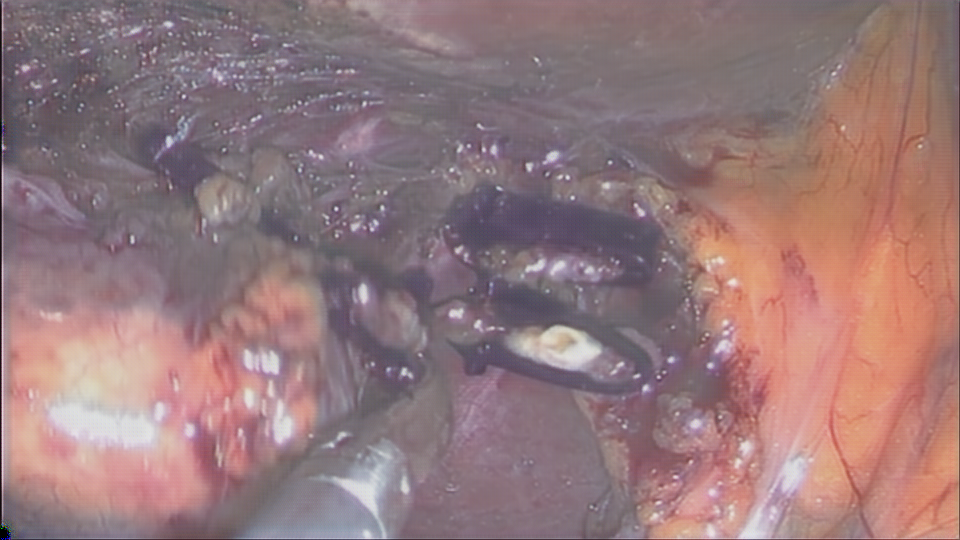
\includegraphics[width=0.33\textwidth]{./images/images_star/f_15075_v3_hs_ep5.png}\label{fig:starimghs1}}
    \hfill
    \subfloat[Generated HS in epoch 20.]{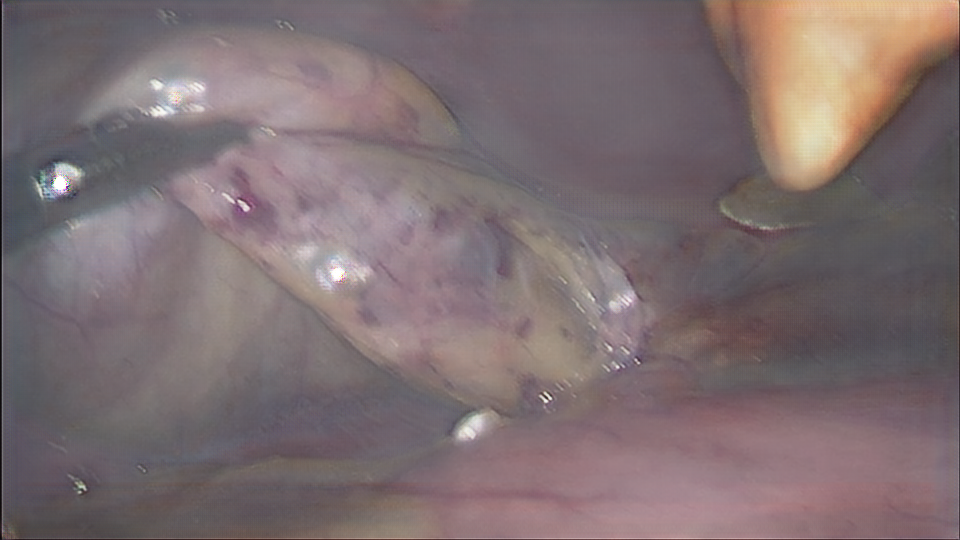
\includegraphics[width=0.33\textwidth]{./images/images_star/f_7450_hs_v4_ep20.png}\label{fig:starimghs2}}
    \hfill
    \subfloat[Generated HS in epoch 30.]{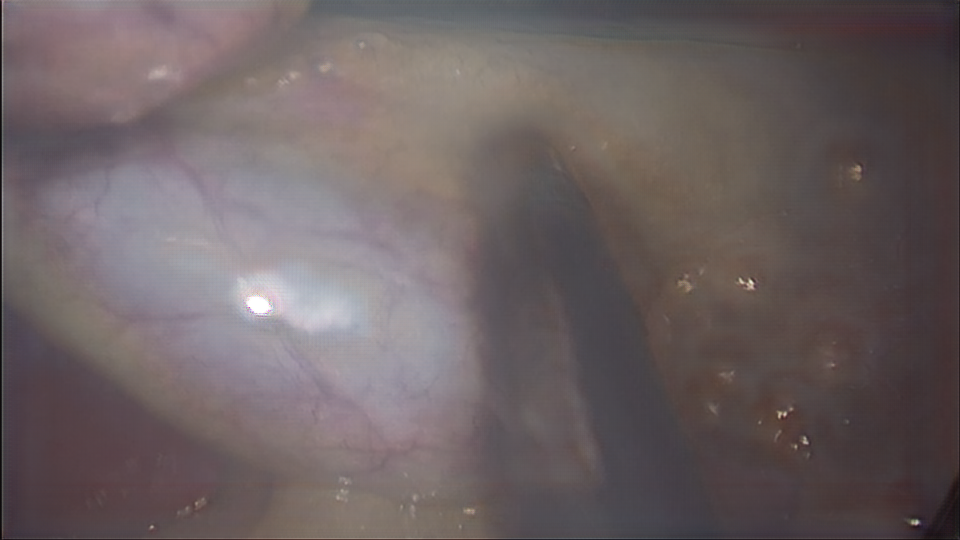
\includegraphics[width=0.33\textwidth]{./images/images_star/f_7450_hs_v2_ep30.png}\label{fig:starimghs3}}
    \vspace{0.5cm}
    \subfloat[Generated SS in epoch 5.]{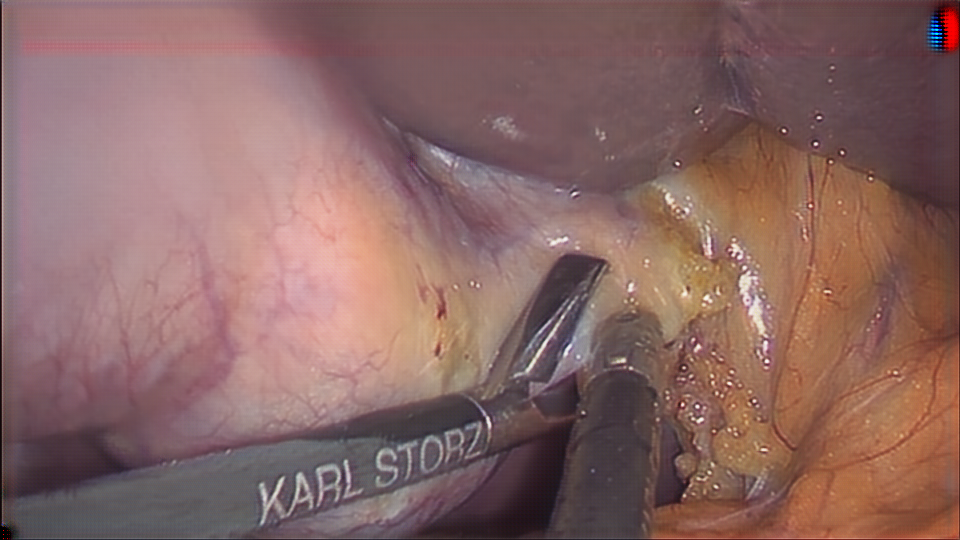
\includegraphics[width=0.33\textwidth]{./images/images_star/f_6100_v3_ms_ep5.png}\label{fig:starimgms1}}
    \hfill
    \subfloat[Generated SS in epoch 20.]{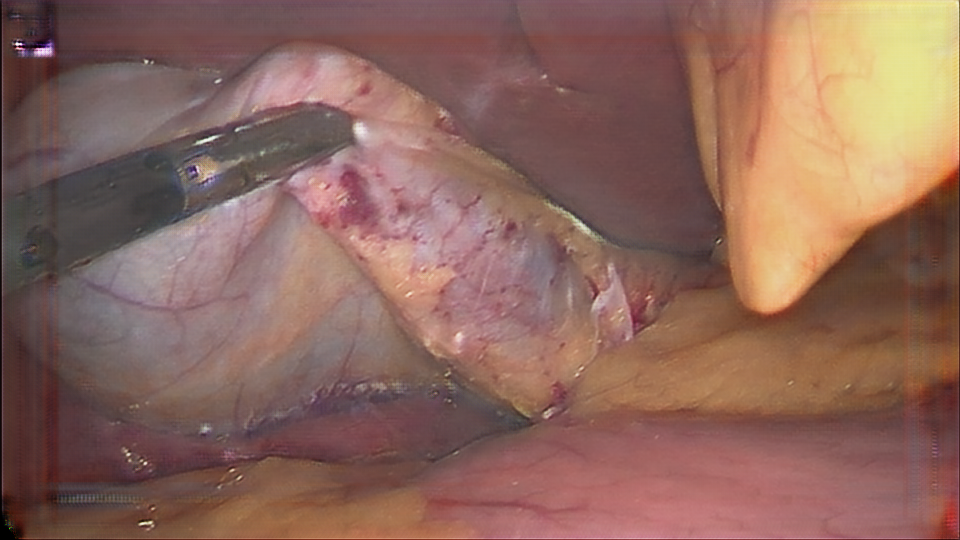
\includegraphics[width=0.33\textwidth]{./images/images_star/f_7825_ms_v4_ep20.png}\label{fig:starimgms2}}
    \hfill
    \subfloat[Generated SS in epoch 30.]{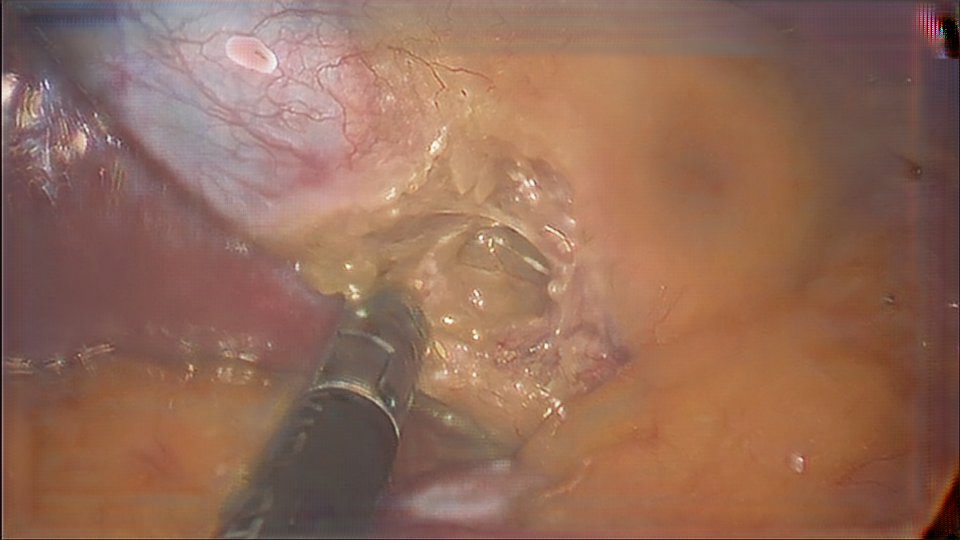
\includegraphics[width=0.33\textwidth]{./images/images_star/f_10375_2_ms_ep30.png}\label{fig:starimgms3}}
     \vspace{0.5cm}
    \caption[Generated images StarGAN]{Display of the images generated heavy-smoke (HS) and slight-smoke (SS) during training the StarGAN at different epochs.}\label{fig:star_showcase}
\end{figure}

%\clearpage
\FloatBarrier
\section{Augmenting data with artificial smoke images}\label{experiment_enhance1}
The generated images are intended to be integrated into the segmentation process to improve its performance.
The baseline will be explained first to enable a comparison between the segmentation results obtained with the generated images and those obtained using the baseline segmentation.
\paragraph{Baseline configuration} The baseline configuration involves the use of a DeepLabv3+ for semantic segmentation.
The DeepLab architecture is constructed as described in section \ref{dlv3_section}.
The baseline approach was implemented using a batch size of 18 and a learning rate of 0.0001.
The Lovász loss function was employed as loss function, as it has been shown to be effective for semantic segmentation tasks.
To further improve training, the one-cycle scheduler was utilized to adjust the learning rate during the course of the training process with a percentage start of 0.05.
Finally, the Adam optimizer was selected with beta values of $0.9$ for $\beta_1$ and 0.999 for $\beta_2 $.
To achieve better results, the model parameters of DeepLabv3+ are loaded from a model pre-trained on the Cityscapes \cite{cordts2016cityscapes} dataset.
Furthermore, a resnet-101 as introduced in \cite{He2015} is used as backbone for the DeepLabV3+.\\
For training and validation, the images are resized to $912\times513$ for computational reasons.
In addition to resizing, the pixel values of the images are standardized, meaning they have a mean of zero and a standard deviation of one.
This can help prevent numerical instability during training and give equal importance to all features, which results in more accurate predictions.%quelle zu standardization
This is done by subtracting the mean value from each pixel and then dividing by the standard deviation. 
The mean and standard deviation are calculated from the pixel values of the used training dataset.
These values are shown in Table \ref{std_mean_table} for the images of the used videos.\\
\begin{table}[b]\vspace{1ex}
    \centering
    \caption[Mean and standard deviation]{Mean and standard deviation for each channel.\label{std_mean_table}}
    \begin{tabular*}{15cm}{l|@{\extracolsep\fill}cccc}
    &\multicolumn{3}{c}{Normalization values} \\
    & Red channel & Green channel & Blue channel  \\\hline
    %\multirow{2}*%{\rotatebox{90}{}}\multirow{6}*{\rotatebox{90}{Domain}}
    Mean & 0.51948161  & 0.38390668 & 0.35970329 \\%\cline{2-6}
    standard deviation & 0.18273795 &  0.15816768 &  0.15964756\\\hline
    \end{tabular*}
    \captionsetup{justification=centering}
\vspace{2ex}\end{table}
The DeepLabv3+ is trained with each of the 6 folds for 50 epochs, with a validation epoch after every 10th epoch, where the model is then used to make predictions for the omitted video to test performance.
\begin{figure}[bt]
    \centering
    \subfloat[mIoU of baseline over all domains.]{\includegraphics[width=0.49\textwidth]{./images/experiment1/ad_miou_bl.pdf}\label{fig:ioublad}}
    \hfill
    \subfloat[mIoU of baseline for heavy-smoke domain.]{\includegraphics[width=0.49\textwidth]{./images/experiment1/hs_miou_bl.pdf}\label{fig:ioublhs}}
    
    \vspace{0.5cm}
    
    \subfloat[mIoU of GI over all domains.]{\includegraphics[width=0.49\textwidth]{./images/experiment1/ad_miou_gi.pdf}\label{fig:ioublss}}
    \hfill
    \subfloat[mIoU of GI for heavy-smoke domain.]{\includegraphics[width=0.49\textwidth]{./images/experiment1/hs_miou_gi.pdf}\label{fig:ioublhs}}
    
    \caption{Comparison of the mIoU values in the validation steps of the baseline and with generated images (GI).}\label{fig:segment_bl}
\end{figure}
%beschreiben wo konvergiert (vlt dass bei hs später konvergiert)

%kurvenverläufe noch mehr beschreiben (auch bei fid und ssim)

\paragraph{Integration of the generated images} Integration of the generated images is done as defined in section \ref{seg_improve_gen}.
The generated images used for this process are the ones resulting from the CycleGAN experiment from epoch 20 as described in section \ref{cyclegan_experiment}, because this configuration has yielded the best images.
A distribution of 50\% heavy-smoke and 50\% no-smoke images was defined as the target ratio.
To achieve this ratio, random images of the no-smoke domain are replaced with their corresponding counterparts in each epoch.
Otherwise, the training is defined as described in the baseline.\\
Figure \ref{fig:segment_bl} shows the progression of mIoU for the baseline compared to the integration of generated images (GI) in all domains and in the heavy-smoke domain.
It can be observed that the images in heavy-smoke domain are segmented less accurate than in all domains.  
Furthermore, compared to the baseline, the segmentation with GI converges faster in the heavy-smoke domain than the baseline.
In the case of all domains, it is to be observed that the mIoU of the segmentation with GI does not improve as fast as the baseline between epoch 10 and 30.
However there is a more significant increase towards the end of the training process than in the baseline.\\
Additionally, the mean Dice coefficient was employed as an evaluation metric.
Tables \ref{iou_exp1_table} and \ref{dice_exp1_table} show the results of the baseline method compared to those of the segmentation approach using generated images to evaluate the performance of the proposed method.
The metrics, including mIoU and mDice, are computed for all images within each fold and are evaluated after training the models 50 epochs.
Moreover, the frames are categorized into the three domains: no-smoke, heavy-smoke, and slight-smoke and the metrics are computed separately for each domain.
\begin{table}[bt]\vspace{1ex}
    \centering
    \caption[mIoU comparison experiment 1]{Comparison of segmentation baseline (BL) and with generated images (GI) by mIoU. The values are rounded to one decimal place.\label{iou_exp1_table}}
    \begin{tabular}{ll|cc|cc|cc|cc}
       && \multicolumn{2}{c|}{All domains} & \multicolumn{2}{c|}{No-smoke} & \multicolumn{2}{c|}{Slight-smoke} & \multicolumn{2}{c}{Heavy-smoke} \\
       && BL & GI & BL & GI & BL & GI & BL & GI \\
      \hline
      \multirow{6}*{\rotatebox{90}{Fold}}
      &1 & 57.9 & 58.7 & 53.2 & 53.8 & 52.4 & 55.4 & 45.0 & 45.0 \\
      &2 &51.5 & 54.3 & 45.0 & 45.7 & 39.7 & 42.2 & 38.1 & 39.8 \\
      &3 &53.7& 53.8 & 53.5 & 54.1 & 36.4 & 35.0 & 38.7 & 39.1 \\
      &4 &58.6 & 59.1 & 58.8 & 59.9 & 41.5 & 40.2 & 38.2 & 38.9 \\
      &5 &61.2 & 62.4 & 61.1 & 63.3 & 39.6 & 41.0 & 30.3 & 30.1 \\
      &6 &70.6 & 70.3 & 70.1 & 69.2 & 48.7 & 48.7 & 48.6 & 48.7 \\
      \hline
      &Mean &58.9 & 59.8 & 56.9 & 57.7 & 43.1 & 43.7 & 39.8 & 40.3 \\
    \end{tabular}
    \captionsetup{justification=centering}
\end{table}
\begin{table}[bt]\vspace{1ex}
    \centering
    \caption[mDice comparison experiment 1]{Comparison of segmentation baseline (BL) and with generated images (GI) by mDice coefficient. The values are rounded to one decimal place.\label{dice_exp1_table}}
    \begin{tabular}{ll|cc|cc|cc|cc}
       && \multicolumn{2}{c|}{All domains} & \multicolumn{2}{c|}{No-smoke} & \multicolumn{2}{c|}{Slight-smoke} & \multicolumn{2}{c}{Heavy-smoke} \\
       && BL & GI & BL & GI & BL & GI & BL & GI \\
      \hline
      \multirow{6}*{\rotatebox{90}{Fold}}
      &1 & 70.0 & 70.9  & 63.8 & 64.3 & 63.9 &66.3 & 55.5 & 55.1 \\
      &2 & 65.4&68.0   & 57.4 & 57.6 &51.0 & 53.8 & 48.9 & 50.6 \\
      &3 &66.4 &66.5  & 65.3 & 66.2 & 44.4 & 43.1 & 49.4 & 49.6 \\
      &4 &71.9 &72.6  & 71.7 & 73.3 & 50.6 & 49.4 & 48.1 & 48.9 \\
      &5 &74.3 &75.3  & 71.8 & 73.9 & 49.3 & 49.3 & 38.7 & 38.5 \\
      &6 & 82.2&81.9  & 81.0 & 80.3 & 56.0 & 55.9 & 57.4 & 57.6 \\
      \hline
      &Mean & 71.7 &72.5  & 68.5 & 69.3 & 52.5 & 53.0 & 49.6 & 50.1 \\
    \end{tabular}
    \captionsetup{justification=centering}
\end{table}
Table \ref{iou_exp1_table} illustrates the comparison between generated images and the baseline with respect to mIoU, demonstrating an improvement in all domains combined and also in each sub-domain individually.
Specifically, the mIoU is increased by 1.44\% for all domains, 1.15\% for the heavy-smoke domain, 1.57\% for the slight-smoke domain, and 1.26\% for the no-smoke domain.
Table \ref{dice_exp1_table} presents the comparison in terms of the Dice coefficient, indicating an improvement over all domains of 1.16\%, 0.83\% in the heavy-smoke domain, 0.87\% in the slight-smoke domain, and 1.15\% in the no-smoke domain.
It is to be noted, that the reported improvements are calculated with the absolute values of the metrics and are rounded afterward.
A slight improvement can be observed in almost every comparison of the basline with the generated images.
However, there are exceptions.
For example, the mean Dice coefficient in the slight-smoke domain is only improved for fold 1 and 2 compared to the baseline.\\
\begin{figure}[bt]
    \centering
    \subfloat[Original image.]{\includegraphics[width=0.24\textwidth]{./images/experiment1/f_43575_org_v5.png}\label{fig:ex1_im1}}
    \hfill
    \subfloat[Ground truth.]{\includegraphics[width=0.24\textwidth]{./images/experiment1/43575_mask_color.png}\label{fig:ex1_gt1}}
    \hfill
    \subfloat[Prediction BL.]{
\includegraphics[width=0.24\textwidth]{./images/experiment1/mask_pred_43575_wogen.png}\label{fig:ex1_wo1}}
    \hfill
    \subfloat[Prediction GI.]{
\includegraphics[width=0.24\textwidth]{./images/experiment1/mask_pred_43575_wgen.png}\label{fig:ex1_w1}}
    \vspace{0.3cm}
    \subfloat[Original image.]{\includegraphics[width=0.24\textwidth]{./images/experiment1/f_21025_1.png}\label{fig:ex1_im2}}
    \hfill
    \subfloat[Ground truth.]{\includegraphics[width=0.24\textwidth]{./images/experiment1/21025_mask_color.png}\label{fig:ex1_gt2}}
    \hfill
    \subfloat[Prediction BL.]{
\includegraphics[width=0.24\textwidth]{./images/experiment1/mask_pred_21025_wogen.png}\label{fig:ex1_wo2}}
    \hfill
    \subfloat[Prediction GI.]{
\includegraphics[width=0.24\textwidth]{./images/experiment1/mask_pred_21025_wgen.png}\label{fig:ex1_w2}}
    \vspace{0.3cm}    
    \subfloat[Original image.]{\includegraphics[width=0.24\textwidth]{./images/experiment1/f_10475_v4.png}\label{fig:ex1_im3}}
    \hfill
    \subfloat[Ground truth.]{\includegraphics[width=0.24\textwidth]{./images/experiment1/10475_mask_color.png}\label{fig:ex1_gt3}}
    \hfill
    \subfloat[Prediction BL.]{\includegraphics[width=0.24\textwidth]{./images/experiment1/mask_pred_10475_wogen.png}\label{fig:ex1_wo3}}
    \hfill
    \subfloat[Prediction GI.]{\includegraphics[width=0.24\textwidth]{./images/experiment1/mask_pred_10475_wgen.png}\label{fig:ex1_w3}}
    \vspace{0.3cm}
    \caption[Segmentation results experiment 1]{Visualization of three images with ground truth segmentation masks, comparing the prediction with generated images (GI) and without (BL).}\label{fig:ex1_showcase}
\end{figure}
Next, the impact of the generated images on the segmentation will be examined based on examples.
The ground truth masks were color-coded for improved visualization. 
When comparing the prediction of the images shown in Figures \ref{fig:ex1_im1} and \ref{fig:ex1_im3} before and after training with generated images, an improvement in shaft recognition can be observed. 
It should be noted that false positives here also increase, as there is no PE-Forceps Tip labeled at the end of the shaft in the original mask shown in Figure \ref{fig:ex1_gt3}.
However, the basline segmentation predicts the occurence of a PE-Forceps Tip (highlighted in green). This is further emphasized by training with generated images as even more pixels are classified as PE-Forceps Tip.
The interference in the bottom left corner of the image displayed in Figure \ref{fig:ex1_im1} is better compensated, but part of the non-shaft region in the corner is also recognized as a shaft. 
In the predicted segmentation masks shown in Figures \ref{fig:ex1_wo2} and \ref{fig:ex1_w2}, there are fewer false detections of non-existing surgical instruments for the segmentation trained with generated images, but no significant improvement in the overall segmentation.
\FloatBarrier
\section{GenSegNet}\label{gen_seg_exp12}
To generate even more challenging smoke images for segmentation and to simultaneously train the segmentation model on them, the proposed GenSegNet architecture described in section \ref{seg_improve_gen} is utilized.
As a total of five networks need to collaborate in this process, the images must be further down-scaled to enable efficient computation.
The chosen resolution is $512\times288$, because it is in a 16:9 aspect ratio like the original images.
The dataset for GenSegNet provides the images normalized with mean and standard deviation of the dataset for segmentation, as well as in the range of [-1,1] for CycleGAN.
It is to be noted that the translation of the CycleGAN results in images with a value range of [-1,1]. 
Therefore, prior to being used by the segmentation network, the images must first be rescaled to the standard pixel value range and then re-standardized.\\
As the CycleGAN needs to be pre-trained to avoid producing images that do not match the segmentation masks, the experiment described in section \ref{cyclegan_experiment} is repeated with a reduced resolution of $512\times288$.
The model parameters of the CycleGAN used in GenSegNet correspond to the parameters of a training until epoch 20 of this setup.
For the same reason, a new baseline of the DeepLabv3+ has to be trained.
This segmentation training is the same as the baseline described in section \ref{experiment_enhance1}, except the resizing is changed to the resolution of $512\times288$.
The DeepLabv3+ in GenSegNet takes the model parameters of the segmentation baseline in epoch 20 to continue its training with the integration of CycleGAN.
In the GenSegNet the segmentation network is then trained another 30 epochs to achieve the same amount of training steps as in the baseline.
To achieve comparable results also the parameters of the Adam optimizer and the scheduler for the segmentation training are also taken from epoch 20.\\
\paragraph{Hyperparameters} The hyperparameters for the GenSegNet are experimentally determined as follows.
A learning rate of 0.0001 is chosen for training the DeepLabv3+.
The CycleGAN is trained with a fixed learning rate of 0.0001.
A batch size of 3 is used due to computational reasons.
As mentioned the model is trained for 30 epochs after the pre-training of 20 epochs.
The lambda values are increased to 8 for identity loss and to 20 for cycle-consistency loss to prevent difficult-to-segment images from being generated by altering the overall structure of the image.
Optimizer and loss functions of both models are chosen as stated in the previous experiments described in section \ref{cyclegan_experiment} and \ref{experiment_enhance1}. % evtl ref
The lambda value $\lambda_{\text{seg}}$, which determines the influence the segmentation has on the image translation process, is set to 0.1.\\
Training the GenSegNet is done with six folds, including five of the six videos, for six-fold cross-validation.
The model parameters of CycleGAN and DeepLabv3+ are loaded from the pre-training of the models trained on data of the corresponding fold.\\
\begin{figure}[bt]
    \centering
    \subfloat[Generator loss.]{\includegraphics[width=0.33\textwidth]{./images/seggan_plots/seggan_gen_hs.pdf}\label{fig:gen_seggan}}
    \hfill
    \subfloat[Discriminator loss.]{\includegraphics[width=0.33\textwidth]{./images/seggan_plots/seggan_disc_hs.pdf}\label{fig:disc_seggan}}
    \hfill
    \subfloat[Segmentation loss.]{\includegraphics[width=0.33\textwidth]{./images/seggan_plots/seggan_gp.pdf}\label{fig:gp_seggan}}
    \caption[GenSegNet loss curves]{Display of the generator (a) and discriminator (b) loss of the heavy-smoke domain in the CycleGAN in GenSegNet during training.
    (c) shows the progress of the segmentation reward for the generated images.}\label{fig:gen_disc_genseg}
\end{figure}
Figure \ref{fig:gp_seggan} shows a decline in the segmentation reward over the course of the training.
It exhibits a slight oscillation and stagnates after epoch 20 in training the GenSegNet.
An increase in the generator loss in Figure \ref{fig:gen_seggan} and a decrease in discriminator loss in Figure \ref{fig:disc_seggan} can be observed.
In this case, the loss values for the generator are higher and for the discriminator lower compared to training the CycleGAN on its own.
Furthermore, the loss values of both sub-networks oscillate stronger than in the CycleGAN training described in section \ref{cyclegan_experiment}.\\
\begin{figure}[bt]
    \centering
    \subfloat[]{\includegraphics[width=0.49\textwidth]{./images/seggan_plots/seggan_fid.pdf}\label{fig:fid_seggan}}
    \hfill
    \subfloat[]{\includegraphics[width=0.49\textwidth]{./images/seggan_plots/seggan_ssim.pdf}\label{fig:fid_seggan}}
    \caption[FID and SSIM in GenSegNet]{Display of FID (a) and SSIM (b) during training the GenSegNet.}\label{fig:fid_ssim_genseg}
\end{figure}
Next, the FID and SSIM values shown in Figure \ref{fig:fid_seggan} and \ref{fig:fid_seggan} are examined during training. 
It can be observed that there is no clear improvement in both metrics, and they fluctuate significantly.
However, a slight improvement can be noticed towards the end of the training.\\
\begin{figure}[bt]
    \centering
    \subfloat[]{\includegraphics[width=0.33\textwidth]{./images/Seggan_images/f_11975_v3_ep28.png}\label{fig:ex2_1}}
    \hfill
    \subfloat[]{\includegraphics[width=0.33\textwidth]{./images/Seggan_images/f_12525.png}\label{fig:ex2_2}}
    \hfill
    \subfloat[]{\includegraphics[width=0.33\textwidth]{./images/Seggan_images/f_34450_v2.png}\label{fig:ex2_3}}
    \vspace{0.3cm}
    \subfloat[]{\includegraphics[width=0.33\textwidth]{./images/Seggan_images/f_24550_v2.png}\label{fig:ex2_4}}
    \hfill
    \subfloat[]{\includegraphics[width=0.33\textwidth]{./images/Seggan_images/f_15075_v2.png}\label{fig:ex2_5}}
    \hfill
    \subfloat[]{\includegraphics[width=0.33\textwidth]{./images/Seggan_images/f_39925_v2.png}\label{fig:ex2_6}}

    \subfloat[]{\includegraphics[width=0.33\textwidth]{./images/Seggan_images/f_24550_org.png}\label{fig:ex2_7}}
    \hfill
    \subfloat[]{\includegraphics[width=0.33\textwidth]{./images/Seggan_images/f_15075_org.png}\label{fig:ex2_8}}
    \hfill
    \subfloat[]{\includegraphics[width=0.33\textwidth]{./images/Seggan_images/f_39925_org.png}\label{fig:ex2_9}}
    \caption[Generated images GenSegNet]{Display of generated heavy-smoke images in GenSegNet. (g)-(i) show the original images on which the generated images (d)-(f) are based on.}\label{fig:ex2_img_showcase}
\end{figure}
Figure \ref{fig:ex2_img_showcase} displays images generated during the training of GenSegNet. 
Heavy smoke is evident.
In the images seen in Figures \ref{fig:ex2_4}, \ref{fig:ex2_5}, and \ref{fig:ex2_6} its intensity varies across different regions of the image. 
Particularly, it appears to be more pronounced around the instruments. 
Additionally, increased artifact formation can be observed as seen in Figures \ref{fig:ex2_2} and \ref{fig:ex2_3}, especially in areas with reflections.
The overall structure of the images remains as in the original images.\\
\begin{figure}[bt]
    \centering
    \subfloat[mIoU of baseline over all domains.]{\includegraphics[width=0.49\textwidth]{./images/seggan_plots/bl_klein_ad_iou.pdf}\label{fig:ioublad2}}
    \hfill
    \subfloat[mIoU of baseline for heavy-smoke domain.]{\includegraphics[width=0.49\textwidth]{./images/seggan_plots/bl_klein_hs_iou.pdf}\label{fig:ioublhs2}}
    
    \vspace{0.5cm}
    
    \subfloat[mIoU of GenSegNet for all domains.]{\includegraphics[width=0.49\textwidth]{./images/seggan_plots/seggan_iou_ad.pdf}\label{fig:iougensegad2}}
    \hfill
    \subfloat[mIoU of GenSegNet for heavy-smoke domain.]{\includegraphics[width=0.49\textwidth]{./images/seggan_plots/seggan_iou_hs.pdf}\label{fig:iougenseghs2}}
    
    \caption[Comparison of mIoU in GenSegNet]{Display of the mIoU in the validation steps of the baseline training compared to the baseline.}\label{fig:segment_bl_comp}
\end{figure}
Furthermore, the mIoU values of the GenSegNet training are compared with the baseline across all domains and specifically in the heavy-smoke domain in Figure \ref{fig:segment_bl_comp}.
As the baseline is used as pre-trained model for the segmentation from epoch 20 onwards the 30 epochs depicted for GenSegNet are compared to the last 30 epochs of the baseline training.
For the curve trends in all domains, a similar pattern can be observed, except for fold 6, where GenSegNet shows a sharp increase followed by a rapid decrease.
It is also worth noting that folds 1-3 exhibits stronger fluctuations in GenSegNet (Fig. \ref{fig:iougensegad2}) compared to the baseline (Fig. \ref{fig:ioublad2}).
In the heavy smoked domain, the baseline shows a deterioration in performance for fold 2, 5, and 6 starting from epoch 30 (Fig. \ref{fig:ioublhs2}).
In GenSegNet, folds 2 and 5 show improvement in the heavy-smoke domain throughout the training, while fold 6 still exhibits a decline (Fig. \ref{fig:iougenseghs2}). 
Fold 1, 3, and 4 have a similar curve pattern in both training setups.
\begin{table}[bt]\vspace{1ex}
    \centering
    \captionsetup{justification=centering}
    \caption[mIoU comparison experiment 2]{Comparison of segmentation baseline (BL) and with GenSegNet (GS) by mIoU. It is to be noted that the values are rounded to one decimal place.\label{iou_exp2_table}}
    \begin{tabular}{ll|cc|cc|cc|cc}
       && \multicolumn{2}{c|}{All domains} & \multicolumn{2}{c|}{No-smoke} & \multicolumn{2}{c|}{Slight-smoke} & \multicolumn{2}{c}{Heavy-smoke} \\
       && BL & GS & BL & GS & BL & GS & BL & GS \\
      \hline
      \multirow{6}*{\rotatebox{90}{Fold}}
      &1 &54.3&52.6&50.9&52.0& 46.2&42.6&40.7 & 39.2\\
      &2 &49.6&50.7&42.1 &42.4&37.2 &42.0& 39.4& 41.3\\
      &3 &52.6&52.6& 52.4&51.2&39.6 &37.7&38.4 & 39.5\\
      &4 &51.6&50.0&53.0 &50.8& 40.2&41.6&37.3 & 36.5\\
      &5 &52.2&54.8&53.4 &55.6&37.2 &40.2& 28.2&29.7\\
      &6 &64.1&60.6&64.6 &62.0& 45.8&44.1&42.9 & 41.4\\
      \hline
      &Mean &54.1 & 53.6 & 52.7 & 52.3 & 41.0 &41.4 & 37.8 &  37.9\\
    \end{tabular}
\end{table}
The values were calculated without rounding and the results were rounded to two decimal places.
In Table \ref{iou_exp2_table}, it is evident that the mIoU decreases by 0.98\% in all domains and by 0.84\% in the no-smoked domain by using the GenSegNet compared to the baseline. 
However, there is an improvement of 0.76\% in the slight-smoke domain and 0.28\% in the heavy-smoked domain.
% ad 1,009815 verschl
% hs 1,002798 verb
% ss 1,0076444 verb
% ns 1,008396 verschl
\begin{table}[bt]\vspace{1ex}
    \centering
    \captionsetup{justification=centering}
    \caption[mDice comparison experiment 2]{Comparison of segmentation baseline (BL) and with GenSegNet (GS) by mDice coefficient. It is to be noted that the values are rounded to one decimal place.\label{dice_exp2_table}}
    \begin{tabular}{ll|cc|cc|cc|cc}
       && \multicolumn{2}{c|}{All domains} & \multicolumn{2}{c|}{No-smoke} & \multicolumn{2}{c|}{Slight-smoke} & \multicolumn{2}{c}{Heavy-smoke} \\
       && BL & GS & BL & GS & BL & GS & BL & GS \\
      \hline
      \multirow{6}*{\rotatebox{90}{Fold}}
      &1 &67.7&66.4&62.4&63.2&58.4&54.3&51.1& 49.7\\
      &2 &64.0&65.1&54.1&54.2&48.8&53.5&50.1& 52.5\\
      &3 &65.6&65.5&64.3&63.1&49.3&47.5&49.3& 50.5\\
      &4 &65.6&64.0&66.8&64.5&49.1&50.3&47.5& 46.3\\
      &5 &65.0&67.1&63.7&65.3&46.8&49.1&36.5& 37.9\\
      &6 &77.1&74.1&76.4&74.5&54.0&52.3&52.9& 51.3\\
      \hline
      &Mean & 67.5 & 67.0 & 64.6 & 64.1 &51.1 & 51.2 & 47.9 & 48.0 \\
    \end{tabular}
\end{table}
Similarly, the mDice metric shows improvements for the GenSegNet in the slight-smoke and heavy-smoke domains, while there is a deterioration in the other domains, shown in Table \ref{dice_exp2_table}.
The exact values indicate a 0.71\% degradation in all domains and a 0.75\% degradation in the no-smoke domain. 
However, there is an improvement of 0.22\% in the slight-smoke domain and 0.24\% in the heavy-smoke domain.
% ad 1,0070679 verschl
% hs 1,0023552 verb
% ss 1,0022114 verb
% ns 1,0074614 verschl
% -> in ad iou in 3 werten besser und drei schlechter
% -> man sieht für manche folds hat es besser funktioniert als für andere
% -> vor allem in fold 6 eine deutliche verschlechterung -> wie auch in den grafen aus ... zu erkennen


\begin{figure}[bt]
    \centering
    \subfloat[Original image.]{\includegraphics[width=0.24\textwidth]{./images/seggan_mask/f_16925v7org.png}\label{fig:ex3_im1}}
    \hfill
    \subfloat[Ground truth.]{\includegraphics[width=0.24\textwidth]{./images/seggan_mask/16925_mask_color_v7.png}\label{fig:ex3_gt1}}
    \hfill
    \subfloat[Prediction BL.]{\includegraphics[width=0.24\textwidth]{./images/seggan_mask/mask_pred_16925_pred_bl.png}\label{fig:ex3_wo1}}
    \hfill
    \subfloat[Prediction GenSegNet.]{\includegraphics[width=0.24\textwidth]{./images/seggan_mask/mask_pred_16925_seggan.png}\label{fig:ex3_w1}}
    \vspace{0.3cm}
    \subfloat[Original image.]{\includegraphics[width=0.24\textwidth]{./images/seggan_mask/f_24975orgv7.png}\label{fig:ex3_im2}}
    \hfill
    \subfloat[Ground truth.]{\includegraphics[width=0.24\textwidth]{./images/seggan_mask/24975_mask_color.png}\label{fig:ex3_gt2}}
    \hfill
    \subfloat[Prediction BL.]{\includegraphics[width=0.24\textwidth]{./images/seggan_mask/mask_pred_24975_baseline.png}\label{fig:ex3_wo2}}
    \hfill
    \subfloat[Prediction GenSegNet.]{\includegraphics[width=0.24\textwidth]{./images/seggan_mask/mask_pred_24975_seggen.png}\label{fig:ex3_w2}}
    \vspace{0.3cm}    
    \subfloat[Original image.]{\includegraphics[width=0.24\textwidth]{./images/seggan_mask/f_4275_org.png}\label{fig:ex3_im3}}
    \hfill
    \subfloat[Ground truth.]{\includegraphics[width=0.24\textwidth]{./images/seggan_mask/4275_mask_color_org.png}\label{fig:ex3_gt3}}
    \hfill
    \subfloat[Prediction BL.]{\includegraphics[width=0.24\textwidth]{./images/seggan_mask/mask_pred_4275_bl_v7.png}\label{fig:ex3_wo3}}
    \hfill
    \subfloat[Prediction GenSegNet.]{\includegraphics[width=0.24\textwidth]{./images/seggan_mask/mask_pred_4275_seggen.png}\label{fig:ex3_w3}}
    \vspace{0.3cm} 
    \subfloat[Original image.]{\includegraphics[width=0.24\textwidth]{./images/seggan_mask/f_14825_org.png}\label{fig:ex3_im4}}
    \hfill
    \subfloat[Ground truth.]{\includegraphics[width=0.24\textwidth]{./images/seggan_mask/14825_mask_color_org.png}\label{fig:ex3_gt4}}
    \hfill
    \subfloat[Prediction BL.]{\includegraphics[width=0.24\textwidth]{./images/seggan_mask/mask_pred_14825_bl_v3.png}\label{fig:ex3_wo4}}
    \hfill
    \subfloat[Prediction GenSegNet.]{\includegraphics[width=0.24\textwidth]{./images/seggan_mask/mask_pred_14825_seggan.png}\label{fig:ex3_w4}}
    \caption{Comparison of the predictions of GenSegNet and baseline.}\label{fig:ex3_mask_showcase}
\end{figure}
Figure \ref{fig:ex3_mask_showcase} shows an exemplary comparison of the predictions of GenSegNet and the baseline after training.
The prediction of the original heavy-smoke image in Figure \ref{fig:ex3_im2} improves partly with GenSegNet.
However, it fails to correctly detect the tip of the lower surgical instrument.
The prediction for the image in Figure \ref{fig:ex3_im1}, which is also affected by smoke, generally improves compared to the baseline.
In Figure \ref{fig:ex3_w3}, it can be observed that SegGenNet recognizes the presence of a surgical instrument in the upper right corner but classifies it incorrectly alongside other erroneous predictions.
In the prediction of GenSegNet in Figure \ref{fig:ex3_w4}, a similar problem can be observed. 
While an instrument is detected, it is classified incorrectly in multiple ways without any pixel being correctly classified. 
On the other hand, the baseline segmentation in Figure \ref{fig:ex3_wo4} manages to correctly segment some parts in this case.
%Fragen an tobi
% soll aussage über equilibrium auch hier her?
% evtl auch ohne avg loss von cyclegan?
% satzzeichen bei formaln?
% bei büchern die seiten vo des steht oder die seite wo mans herhat
% validation = test bei uns?
% komma bei tausendern . oder , 
% fragen an tobi: titel passt
% zitieren -> bücher seiten
% 	-> einheitlich so dass nur wichtige infos bei allen
% fragen wie -> soll ich pytorch und seed beschreiben

% beschreiben das maske gray scale ist

% in seg -> scale auf 912x513 wegen effective computation
%###########################
% -> vergleich von hs iou von exp1 und all domains für mit gen und ohne
% -> same bei experiment 2 